\chapter{Why Start Here? Addition and Subtraction}

Addition and subtraction are the building blocks of all mathematical concepts. If we think of math as a language, then addition and subtraction are the alphabet—simple yet powerful tools that help us solve problems, from everyday tasks to complex equations.

Let’s begin by understanding these basic operations deeply. Whether you’re managing your budget, dividing something between friends, or calculating distances, these two operations are always at play.


\section{What Is Addition?}
Addition is the process of combining two or more numbers to get a larger number. Think of it like this:
\begin{itemize}
    \item If you have 3 apples and someone gives you 2 more apples, how many apples do you have in total?
\end{itemize}
This problem is an example of addition: 3 apples + 2 apples = 5 apples.

Let’s look at some other simple examples:
\begin{itemize}
    \item 1 + 1 = 2
    \item 4 + 3 = 7
    \item 10 + 20 = 30
\end{itemize}

Addition works by combining. You start with one number, and as you add more numbers, the total grows.

\subsection{Visualizing Addition}
One of the best ways to understand addition is by using a number line. A number line is a straight line where numbers increase as you move to the right. To add, you simply move to the right by the number you're adding.

For example, if you’re adding 2 + 3, you can start at 2 on the number line and move 3 steps to the right. You’ll land at 5.

\begin{center}
    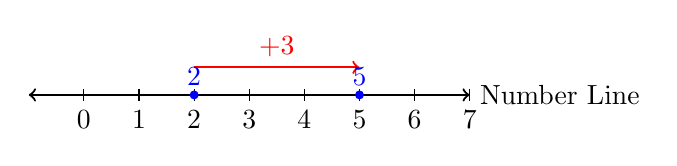
\begin{tikzpicture}[scale=0.7]
        \draw[thick,<->] (-1,0) -- (7,0) node[right] {Number Line};
        \foreach \x in {0,1,...,7}
            \draw (\x,3pt) -- (\x,-3pt) node[below] {\x};
        \draw[red,thick,->] (2,0.5) -- (5,0.5) node[midway,above] {+3};
        \filldraw[blue] (2,0) circle (2pt) node[above] {2};
        \filldraw[blue] (5,0) circle (2pt) node[above] {5};
    \end{tikzpicture}
\end{center}

\section{What Is Subtraction?}
Subtraction is the process of taking one number away from another. If addition is about combining, subtraction is about removing.

For example:
\begin{itemize}
    \item You have 5 apples, and you give 2 away. How many apples are left?
\end{itemize}
This is subtraction: 5 apples - 2 apples = 3 apples.

Other simple examples:
\begin{itemize}
    \item 7 - 4 = 3
    \item 10 - 5 = 5
    \item 15 - 9 = 6
\end{itemize}

Subtraction helps us find out how much is left or how much we need to remove from something.

\subsection{Visualizing Subtraction}
We can also use a number line for subtraction. Instead of moving to the right as we do with addition, we move to the left.

If you’re subtracting 5 - 2, you start at 5 on the number line and move 2 steps to the left. You’ll land at 3.

\begin{center}
    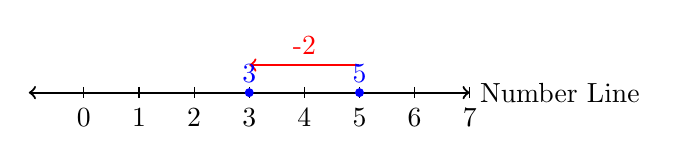
\begin{tikzpicture}[scale=0.7]
        \draw[thick,<->] (-1,0) -- (7,0) node[right] {Number Line};
        \foreach \x in {0,1,...,7}
            \draw (\x,3pt) -- (\x,-3pt) node[below] {\x};
        \draw[red,thick,<-] (3,0.5) -- (5,0.5) node[midway,above] {-2};
        \filldraw[blue] (3,0) circle (2pt) node[above] {3};
        \filldraw[blue] (5,0) circle (2pt) node[above] {5};
    \end{tikzpicture}
\end{center}

\section{Practice Makes Perfect: Let’s Try Some Exercises!}
Now that we understand the basics of addition and subtraction, let’s practice with some simple problems. Remember, the more you practice, the better you’ll get!
\begin{multicols}{2}
    \text{Addition}
    \begin{enumerate}[label=(\alph*)]
        \item $5 + 4 = \underline{\hspace{0.5cm}}$
        \item $7 + 2 = \underline{\hspace{0.5cm}}$
        \item $10 + 6 = \underline{\hspace{0.5cm}}$
        \item $3145 + 1234 = \underline{\hspace{0.5cm}}$
        \item $100 + 1000 = \underline{\hspace{0.5cm}}$
        \item $1234 + 5678 = \underline{\hspace{0.5cm}}$
    \end{enumerate}
    \text{Subtraction}
    \begin{enumerate}[label=(\alph*)]
        \item $8 - 3 = \underline{\hspace{0.5cm}}$
        \item $12 - 5 = \underline{\hspace{0.5cm}}$
        \item $20 - 9 = \underline{\hspace{0.5cm}}$
        \item $32 - 15 = \underline{\hspace{0.5cm}}$
        \item $100 - 50 = \underline{\hspace{0.5cm}}$
        \item $9534 - 1234 = \underline{\hspace{0.5cm}}$
    \end{enumerate}
\end{multicols}

\textbf{Note:} You can use a number line to help you visualize these problems. For example, to solve $5 + 4$, you can draw a number line and move 4 steps to the right from 5.
\noindent
\begin{center}
    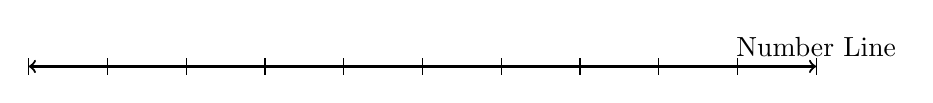
\begin{tikzpicture}
        \draw[thick,<->] (-5,0) -- (5,0) node[above] {Number Line};
        \foreach \x in {-5,-4,...,5}
            \draw (\x,3pt) -- (\x,-3pt);
    \end{tikzpicture}
    \end{center}

\section{Making It Real: Addition and Subtraction in Everyday Life}
Math is everywhere. You use addition and subtraction more often than you think:
\begin{itemize}
    \item \textbf{Shopping:} You bought 3 oranges and added 2 apples to your basket. How many pieces of fruit do you have? That’s 3 + 2 = 5
    \item \textbf{Cooking:} You have 4 cups of flour, but your recipe only calls for 2 cups. How much flour will you have left after using what you need? That’s 4 - 2 = 2 cups left.
    \item \textbf{Traveling:} Your on a 20 mile trip you have traveled 15 miles. How many miles are left to go? That’s 20 - 15 = 5 miles left.
\end{itemize}

Addition and subtraction help you organize, plan, and make decisions in your daily life.

\section{The Properties of Addition and Subtraction}
Now that we’ve mastered the basics, let’s look at some important properties that will help us understand these operations even better:

\subsection{Commutative Property of Addition}
\begin{itemize}
    \item When adding two numbers, the order doesn’t matter.
    \item For example, 3 + 5 is the same as 5 + 3. Both equal 8.
\end{itemize}

\subsection{Associative Property of Addition}
\begin{itemize}
    \item When adding three or more numbers, it doesn’t matter how you group them.
    \item For example, (2 + 3) + 4 = 2 + (3 + 4). Both equal 9.
\end{itemize}

\subsection{Subtraction is not Commutative}
\begin{itemize}
    \item Unlike addition, the order does matter in subtraction.
    \item For example, 5 - 3 is not the same as 3 - 5. One equals 2, and the other equals -2.
\end{itemize}

\section{Breaking It Down: How to Approach Word Problems}
One of the most important ways math shows up in real life is through word problems. Word problems take a real-world situation and ask you to solve it with math.

Here’s a simple strategy to help you:
\begin{enumerate}
    \item Read the problem carefully.
    \item Identify what you’re being asked to find.
    \item Translate the words into numbers (e.g., “two more” means +2).
    \item Write down the math problem.
    \item Solve it!
\end{enumerate}

Let’s try an example:
\subsection{\textbf{Problem:}}
 Sarah has 5 marbles. She finds 3 more marbles. How many marbles does Sarah have now?
\begin{itemize}
  
    \item \textbf{Step 1:} Identify what we know.
    \begin{enumerate}[label=\alph*)]
        \item Sarah starts with 5 marbles.
        \item She finds 3 more.
    \end{enumerate}
    \item \textbf{Step 2:} Write the math problem:
    \begin{enumerate}[label=\alph*)]
        \item 5 + 3 = 8.
    \end{enumerate}
    \item \textbf{Step 3:} Solve it. Sarah now has 8 marbles.
\end{itemize}

\section{Chapter Summary}
\begin{itemize}
    \item Addition is about combining numbers to get a larger total.
    \item Subtraction is about removing numbers to see how much is left.
    \item We can use number lines to help visualize both operations.
    \item These operations are useful in everyday life, from shopping to cooking and traveling.
    \item We learned the commutative and associative properties for addition and why subtraction doesn’t have these properties.
\end{itemize}
\section{Challenge Question}
Mastering addition and subtraction will set the stage for learning more advanced math concepts in the next chapters. Keep practicing, and soon you’ll be ready for the next step: multiplication and division!

\textbf{Note:} You can use a number line to help you visualize these problems. 
\noindent
\begin{center}
    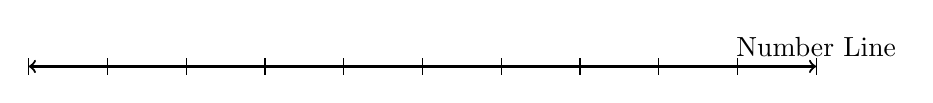
\begin{tikzpicture}
        \draw[thick,<->] (-5,0) -- (5,0) node[above] {Number Line};
        \foreach \x in {-5,-4,...,5}
            \draw (\x,3pt) -- (\x,-3pt);
    \end{tikzpicture}
    \end{center}
    
\begin{enumerate}[label=(\alph*)]  
    \item You have 10 apples. You give 4 apples to your friend, and then you buy 5 more apples. How many apples do you have now?
    \begin{itemize}
        \item $(10 - 4) + 5 = \underline{\hspace{0.5cm}}$
    \end{itemize}
    \item You have 15 candies. You eat 3 candies and then receive 7 more candies from a friend. How many candies do you have now?
    \begin{itemize}
        \item $(15 - 3) + 7 = \underline{\hspace{0.5cm}}$
    \end{itemize}    
    \item You have 20 books. You lend 5 books to a friend and then buy 3 more books. How many books do you have now?
    \begin{itemize}
        \item $(20 - 5) + 3 = \underline{\hspace{0.5cm}}$
    \end{itemize}
    \item You have 30 pencils. You give 10 pencils to your classmates and then find 8 more pencils. How many pencils do you have now?
    \begin{itemize}
        \item $(30 - 10) + 8 = \underline{\hspace{0.5cm}}$
    \end{itemize}
    \item You have 50 stickers. You use 20 stickers and then receive 15 more stickers as a gift. How many stickers do you have now?
    \begin{itemize}
        \item $(50 - 20) + 15 = \underline{\hspace{0.5cm}}$
    \end{itemize}
    \item You have 100 dollars. You spend 40 dollars on groceries and then earn 25 dollars from a part-time job. How much money do you have now?
    \begin{itemize}
        \item $(100 - 40) + 25 = \underline{\hspace{0.5cm}}$
    \end{itemize}
    \item You have 12 cookies. You eat 4 cookies and then bake 10 more cookies. How many cookies do you have now?
    \begin{itemize}
        \item $(12 - 4) + 10 = \underline{\hspace{0.5cm}}$
    \end{itemize}
    \item You have 18 balloons. 6 balloons pop, and then you buy 9 more balloons. How many balloons do you have now?
    \begin{itemize}
        \item $(18 - 6) + 9 = \underline{\hspace{0.5cm}}$
    \end{itemize}
    \item You have 25 marbles. You lose 7 marbles and then find 12 more marbles. How many marbles do you have now?
    \begin{itemize}
        \item $(25 - 7) + 12 = \underline{\hspace{0.5cm}}$
    \end{itemize}
    \item You have 40 candies. You give 15 candies to your friends and then receive 20 more candies. How many candies do you have now?
    \begin{itemize}
        \item $(40 - 15) + 20 = \underline{\hspace{0.5cm}}$
    \end{itemize}
    \item You have 60 pages to read. You read 20 pages and then your teacher assigns 30 more pages. How many pages do you have to read now?
    \begin{itemize}
        \item $(60 - 20) + 30 = \underline{\hspace{0.5cm}}$
    \end{itemize}
\end{enumerate}

